\documentclass[preview]{standalone}

\usepackage{tikz}
%%%%%%%%%%%%%%%%%
%Donut Chart
%%%%%%%%%%%%%%%%%%%%
\def\innerradius{0.7cm}
\def\outerradius{1.9cm}
\pgfmathsetlengthmacro{\centerradius}{(\outerradius + \innerradius)/2}
\pgfmathsetlengthmacro{\donutcenter}{\innerradius/2}
 % The Macro
\newcommand{\donutchart}[1]{
   % Calculate total
   \pgfmathsetmacro{\totalnum}{0}
   \foreach \value/\colour/\name in {#1} {
     \pgfmathparse{\value+\totalnum}
     \global\let\totalnum=\pgfmathresult
   }


  \pgfmathsetmacro{\wheelwidth}{\outerradius-\innerradius}
  \pgfmathsetmacro{\midradius}{(\outerradius+\innerradius)/2}

  \begin{scope}[rotate=90]

    \pgfmathsetmacro{\cumnum}{0}
    \foreach \value/\colour/\name in {#1} {
        \pgfmathsetmacro{\newcumnum}{\cumnum + \value/\totalnum*360}

        \pgfmathsetmacro{\midangle}{-(\cumnum+\newcumnum)/2}

        \filldraw[draw=white,fill=\colour] (-\cumnum:\outerradius) arc (-\cumnum:-(\newcumnum):\outerradius) --
        (-\newcumnum:\innerradius) arc (-\newcumnum:-(\cumnum):\innerradius) -- cycle;

        \fill[darkgray!25] circle (\innerradius);

        \draw node [text=white, font=\bfseries] at (\midangle:{\innerradius+\wheelwidth/2}) {\name};

        %\node[scale=1.0, color=black, font=\bfseries](\innerradius) {A};

        \global\let\cumnum=\newcumnum
    }

  \end{scope}

  }

\begin{document}

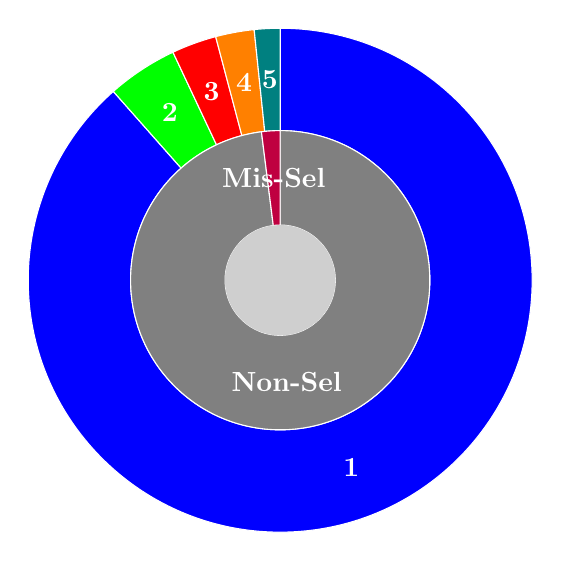
\begin{tikzpicture} 
\def\innerradius{1.9cm}
\def\outerradius{3.2cm}
\pgfmathsetlengthmacro{\centerradius}{(\outerradius + \innerradius)/2}
\pgfmathsetlengthmacro{\donutcenter}{\innerradius/2}

\donutchart{88/blue/1,4.5/green/2, 2.86/red/3, 2.46/orange/4, 1.64/teal/5}

\def\innerradius{0.7cm}
\def\outerradius{1.9cm}
\pgfmathsetlengthmacro{\centerradius}{(\outerradius + \innerradius)/2}
\pgfmathsetlengthmacro{\donutcenter}{\innerradius/2}

 \donutchart{98/gray/Non-Sel,2/purple/Mis-Sel}
\end{tikzpicture}
\end{document}
